\begin{figure}[t]
\centering
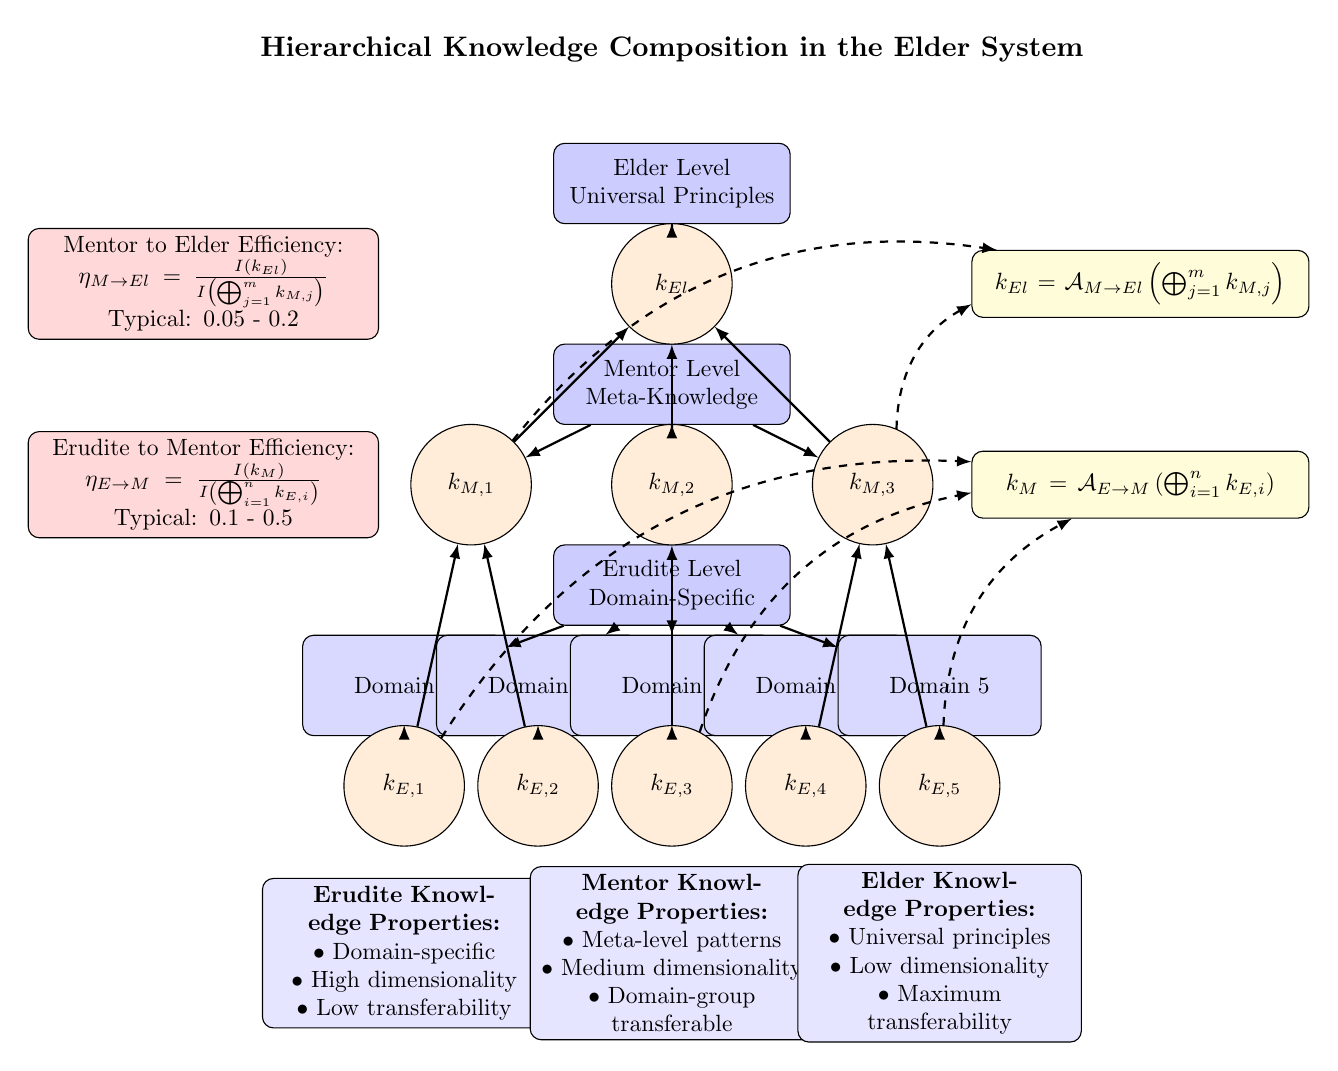
\begin{tikzpicture}[scale=0.85, transform shape]
    % Define styles
    \tikzset{
        level/.style={
            draw,
            fill=blue!20,
            rounded corners,
            minimum width=3.5cm,
            minimum height=1.2cm,
            text width=3.3cm,
            align=center
        },
        domain/.style={
            draw,
            fill=green!15,
            rounded corners,
            minimum width=2cm,
            minimum height=0.8cm,
            text width=1.8cm,
            align=center
        },
        knowledge/.style={
            draw,
            fill=orange!15,
            circle,
            minimum size=1.8cm,
            align=center
        },
        arrow/.style={
            ->,
            thick,
            >=latex
        },
        equation/.style={
            draw,
            fill=yellow!15,
            rounded corners,
            minimum width=5cm,
            minimum height=1cm,
            text width=4.8cm,
            align=center
        }
    }
    
    % Erudite level domains
    \node[level] (erudite) at (0,0) {Erudite Level\\Domain-Specific};
    
    \node[draw, fill=blue!15, rounded corners, minimum width=3cm, minimum height=1.5cm, text width=2.8cm, align=center] (d1) at (-4,-1.5) {Domain 1};
    \node[draw, fill=blue!15, rounded corners, minimum width=3cm, minimum height=1.5cm, text width=2.8cm, align=center] (d2) at (-2,-1.5) {Domain 2};
    \node[draw, fill=blue!15, rounded corners, minimum width=3cm, minimum height=1.5cm, text width=2.8cm, align=center] (d3) at (0,-1.5) {Domain 3};
    \node[draw, fill=blue!15, rounded corners, minimum width=3cm, minimum height=1.5cm, text width=2.8cm, align=center] (d4) at (2,-1.5) {Domain 4};
    \node[draw, fill=blue!15, rounded corners, minimum width=3cm, minimum height=1.5cm, text width=2.8cm, align=center] (d5) at (4,-1.5) {Domain 5};
    
    % Domain knowledge
    \node[knowledge] (k1) at (-4,-3) {$k_{E,1}$};
    \node[knowledge] (k2) at (-2,-3) {$k_{E,2}$};
    \node[knowledge] (k3) at (0,-3) {$k_{E,3}$};
    \node[knowledge] (k4) at (2,-3) {$k_{E,4}$};
    \node[knowledge] (k5) at (4,-3) {$k_{E,5}$};
    
    % Connect domains to knowledge
    \draw[arrow] (d1) -- (k1);
    \draw[arrow] (d2) -- (k2);
    \draw[arrow] (d3) -- (k3);
    \draw[arrow] (d4) -- (k4);
    \draw[arrow] (d5) -- (k5);
    
    % Connect domains to Erudite level
    \draw[arrow] (erudite) -- (d1);
    \draw[arrow] (erudite) -- (d2);
    \draw[arrow] (erudite) -- (d3);
    \draw[arrow] (erudite) -- (d4);
    \draw[arrow] (erudite) -- (d5);
    
    % Mentor level
    \node[level] (mentor) at (0,3) {Mentor Level\\Meta-Knowledge};
    
    % Mentor knowledge groups
    \node[knowledge] (km1) at (-3,1.5) {$k_{M,1}$};
    \node[knowledge] (km2) at (0,1.5) {$k_{M,2}$};
    \node[knowledge] (km3) at (3,1.5) {$k_{M,3}$};
    
    % Connect Erudite knowledge to Mentor knowledge
    \draw[arrow] (k1) -- (km1);
    \draw[arrow] (k2) -- (km1);
    \draw[arrow] (k3) -- (km2);
    \draw[arrow] (k4) -- (km3);
    \draw[arrow] (k5) -- (km3);
    
    % Connect Mentor level to Mentor knowledge
    \draw[arrow] (mentor) -- (km1);
    \draw[arrow] (mentor) -- (km2);
    \draw[arrow] (mentor) -- (km3);
    
    % Elder level
    \node[level] (elder) at (0,6) {Elder Level\\Universal Principles};
    
    % Universal principle
    \node[knowledge] (kel) at (0,4.5) {$k_{El}$};
    
    % Connect Mentor knowledge to Elder knowledge
    \draw[arrow] (km1) -- (kel);
    \draw[arrow] (km2) -- (kel);
    \draw[arrow] (km3) -- (kel);
    
    % Connect Elder level to Elder knowledge
    \draw[arrow] (elder) -- (kel);
    
    % Composition equations
    \node[equation] (e_to_m) at (7,1.5) {$k_M = \mathcal{A}_{E \rightarrow M}\left(\bigoplus_{i=1}^{n} k_{E,i}\right)$};
    \node[equation] (m_to_el) at (7,4.5) {$k_{El} = \mathcal{A}_{M \rightarrow El}\left(\bigoplus_{j=1}^{m} k_{M,j}\right)$};
    
    % Connect to equations
    \draw[arrow, dashed] (k1) to[bend left] (e_to_m);
    \draw[arrow, dashed] (k3) to[bend left] (e_to_m);
    \draw[arrow, dashed] (k5) to[bend left] (e_to_m);
    \draw[arrow, dashed] (km1) to[bend left] (m_to_el);
    \draw[arrow, dashed] (km3) to[bend left] (m_to_el);
    
    % Efficiency measures
    \node[draw, fill=red!15, rounded corners, text width=5cm, align=center] at (-7,1.5) {
        Erudite to Mentor Efficiency:\\
        $\eta_{E \rightarrow M} = \frac{I(k_M)}{I\left(\bigoplus_{i=1}^{n} k_{E,i}\right)}$\\
        Typical: 0.1 - 0.5
    };
    
    \node[draw, fill=red!15, rounded corners, text width=5cm, align=center] at (-7,4.5) {
        Mentor to Elder Efficiency:\\
        $\eta_{M \rightarrow El} = \frac{I(k_{El})}{I\left(\bigoplus_{j=1}^{m} k_{M,j}\right)}$\\
        Typical: 0.05 - 0.2
    };
    
    % Properties
    \begin{scope}[shift={(0,-5.5)}]
        \node[draw, fill=blue!10, rounded corners, text width=4cm, align=center] at (-4,0) {
            \textbf{Erudite Knowledge Properties:}\\
            $\bullet$ Domain-specific\\
            $\bullet$ High dimensionality\\
            $\bullet$ Low transferability
        };
        
        \node[draw, fill=blue!10, rounded corners, text width=4cm, align=center] at (0,0) {
            \textbf{Mentor Knowledge Properties:}\\
            $\bullet$ Meta-level patterns\\
            $\bullet$ Medium dimensionality\\
            $\bullet$ Domain-group transferable
        };
        
        \node[draw, fill=blue!10, rounded corners, text width=4cm, align=center] at (4,0) {
            \textbf{Elder Knowledge Properties:}\\
            $\bullet$ Universal principles\\
            $\bullet$ Low dimensionality\\
            $\bullet$ Maximum transferability
        };
    \end{scope}
    
    % Title
    \node[align=center, font=\bfseries, scale=1.2] at (0,8) {Hierarchical Knowledge Composition in the Elder System};
    
\end{tikzpicture}
\caption{Hierarchical knowledge composition in the Elder system. Domain-specific knowledge at the Erudite level is abstracted to form meta-knowledge at the Mentor level, which is further abstracted to form universal principles at the Elder level. Each abstraction step involves composition through the abstraction operator $\mathcal{A}$, which combines and generalizes knowledge from the lower level. The efficiency of these compositions, measured as the ratio of information content between levels ($\eta_{E \rightarrow M}$ and $\eta_{M \rightarrow El}$), decreases at higher levels of abstraction due to increased generalization. This hierarchical composition structure enables the Elder system to extract progressively more abstract and transferable knowledge, from domain-specific details (high dimensionality, low transferability) to universal principles (low dimensionality, maximum transferability).}
\label{fig:hierarchical_composition}
\end{figure}